\documentclass[11pt]{article}
\usepackage{setspace} 
\usepackage{caption}
\usepackage{subcaption}
\usepackage{amssymb,verbatim,epsfig}
\usepackage{amsmath,setspace}
\usepackage[comma,sort&compress,super]{natbib}
\usepackage{multicol}
\usepackage[usenames,dvipsnames]{color}
\usepackage{url}
\addtolength{\topmargin}{-.8in}
\usepackage{amssymb, amsmath, verbatim, epsfig}
\usepackage{setspace}
\usepackage{lineno}
\usepackage{graphicx}
\graphicspath{ {./images/} }
\linenumbers
\renewcommand {\baselinestretch}{1.}
\topmargin=-1.in
\setlength{\textwidth}{6.5in}
\setlength{\textheight}{9.in}
\setlength{\evensidemargin}{0in}
\setlength{\oddsidemargin}{0in}
\setlength{\topmargin}{-0.4in}

\newcommand{\eq}[1]{Equation\ (\ref{#1})}
\newcommand{\fig}[1]{{\bf Figure \ref{#1}}}
\newcommand{\tab}[1]{Table \ref{#1}}
\newcommand{\et}{{\it et al}}
\newcommand{\sgn}{\text{sgn}}


\usepackage{mathtools}
\DeclarePairedDelimiter\floor{\lfloor}{\rfloor}

\spacing{1}    

\title{\bf 
\vspace{-1in}
Alveus Sci Comm Tech}

\author{Emma Hudock, Kewal Shah, Shannon Royer, Wanrui Xin \\
\text{\small{Schools of Interactive Computing, Civil and Environmental Engineering, and Biological Sciences$^4$}}\\
\text{\small{Georgia Institute of Technology, Atlanta, GA 30332, USA}}}

\begin{document}
\maketitle 


%Type in three keywords to help you give the scope of your overall project
\noindent{\bf Keywords:} \\%see examples given here
Bird feeder, Bird Training, Nonprofit

%This is the section you will do last - it includes a sentence or two from each of the following sections, if you put a star before the section it doesn't give it a number like 1 - introduction as you see below
\section*{Abstract}
Create an automated bird feeder that will help train parrots to say new words or phrases. Twitch, a live streaming website and app, will be the focus of our human-centered design. Viewers will be able to donate, and then a command word or phrase will be given that the parrots should repeat.


\section{Introduction}
Alveus is a nonprofit organization and conservation for animals that have been rescued, are non-releasable, or etc. located in Austin, Texas
. It's founded by Maya Higa, a fairly well-known Twitch streamer. This organization utilizes Twitch to share conservation education (collaborations with larger streamers, live-streaming ,etc.)



\section{Results}
\subsection{Automated Bird Feeder Design}
%In the Results you can reference different figures that you will have at the very end of the report. 
We designed a bird feeder with 54cm and 71cm tall, which is with the 2ft wide, 3ft tall size limitation. The Longest cylinder (part 2) is a place for birds to stand when they pick seed. The end of this cylinder will be inserted with part 1. The other shorter cylinders are used for merging parts. Baffle on part 4 is designed to prevent seed falling and rolling to the ground. We also designed a removable bottom pallet to avoid seed crumbs accumulating. Part 5 and 6 are cuboid with holes which support the plastic container. Part 7 has a wider bottle mouth, we aimed to make filling easier and can be hold up by cuboid.


\section{Discussion}
%The discussion section is for you to discuss the results and the implications they could have for other scientists. 

\subsection{Seed Dispenser Technology}
%Very detailed and boring you can constantly update these as you are working on your project. 
Within the automatic bird feeder, the main technology that will release seeds is a dispenser. There are two possible designs: bottle-shaped or rows, based on canine treat dispensing technology -Figure?-. Experiments and tests will be conducted in order to distinguish which design is more efficient and less problematic. The amount of seeds that can be held at a time inside the dispenser is also an important parameter to keep in mind, as well as how seeds will be filled and refilled in the dispenser.


\subsection{User Interface Remote Button}
%Very detailed and boring you can constantly update these as you are working on your project. 
Our plan is to start with a simple prototype with a user interface button for transmitting a manual signal to the feeder to dispense seeds. From the existing tools, we found that WiFi based Pet feeders have the technology similar to what we want to achieve. We plan to use RasberryPi (\fig{RaspberryPi}), GPIO controllers, Bluetooth, and a Micro SD card {\cite{10.1007/978-981-33-4443-3_15}}. To enforce communication security, TLS/SSL protocol can be used. We explored a similar dog feeder where an Android application was built to communicate through MQTT protocol by using service provided by Paho Android Service. Automatic feeding was performed by connecting an Android application with a server and Smart Dog Feeder through WiFi communication, and they exchange messages with MQTT protocol (\cite{7863048}). In future, we can automate the process of recognizing bird calls (\fig{BirdCalls} and sending a signal to the bird feeder to dispense food. To accomplish that, we did some research and found AudioMoth to be the best option. It is a low-cost acoustic logger which can be used for recognizing different bird call frequencies. It uses a machine learning model to predict species present in a soundscape recording. Each device is able to capture 150–200 hours of audio on one battery charge.



\section{Conclusions}
There are some problems exits on our design. Our design is not accurate and without test. Next semester, we will design a more fitable bird's feeder after several tests, such as support capacity and structural stability.


\section{Acknowledgements} 
This work was supported by the Georgia Tech Vetically Integrated Projects Program. We thank A. Schulz and D. Wu for their guidance. We thank Alveus and C. O'Brien for their assistance with information regarding their four parrots, as well as parameters for the automatic bird feeder.

\bibliographystyle{unsrt}
\bibliography{BIRD_FEEDER}

\pagebreak

\begin{figure}[htp]
    \centering
    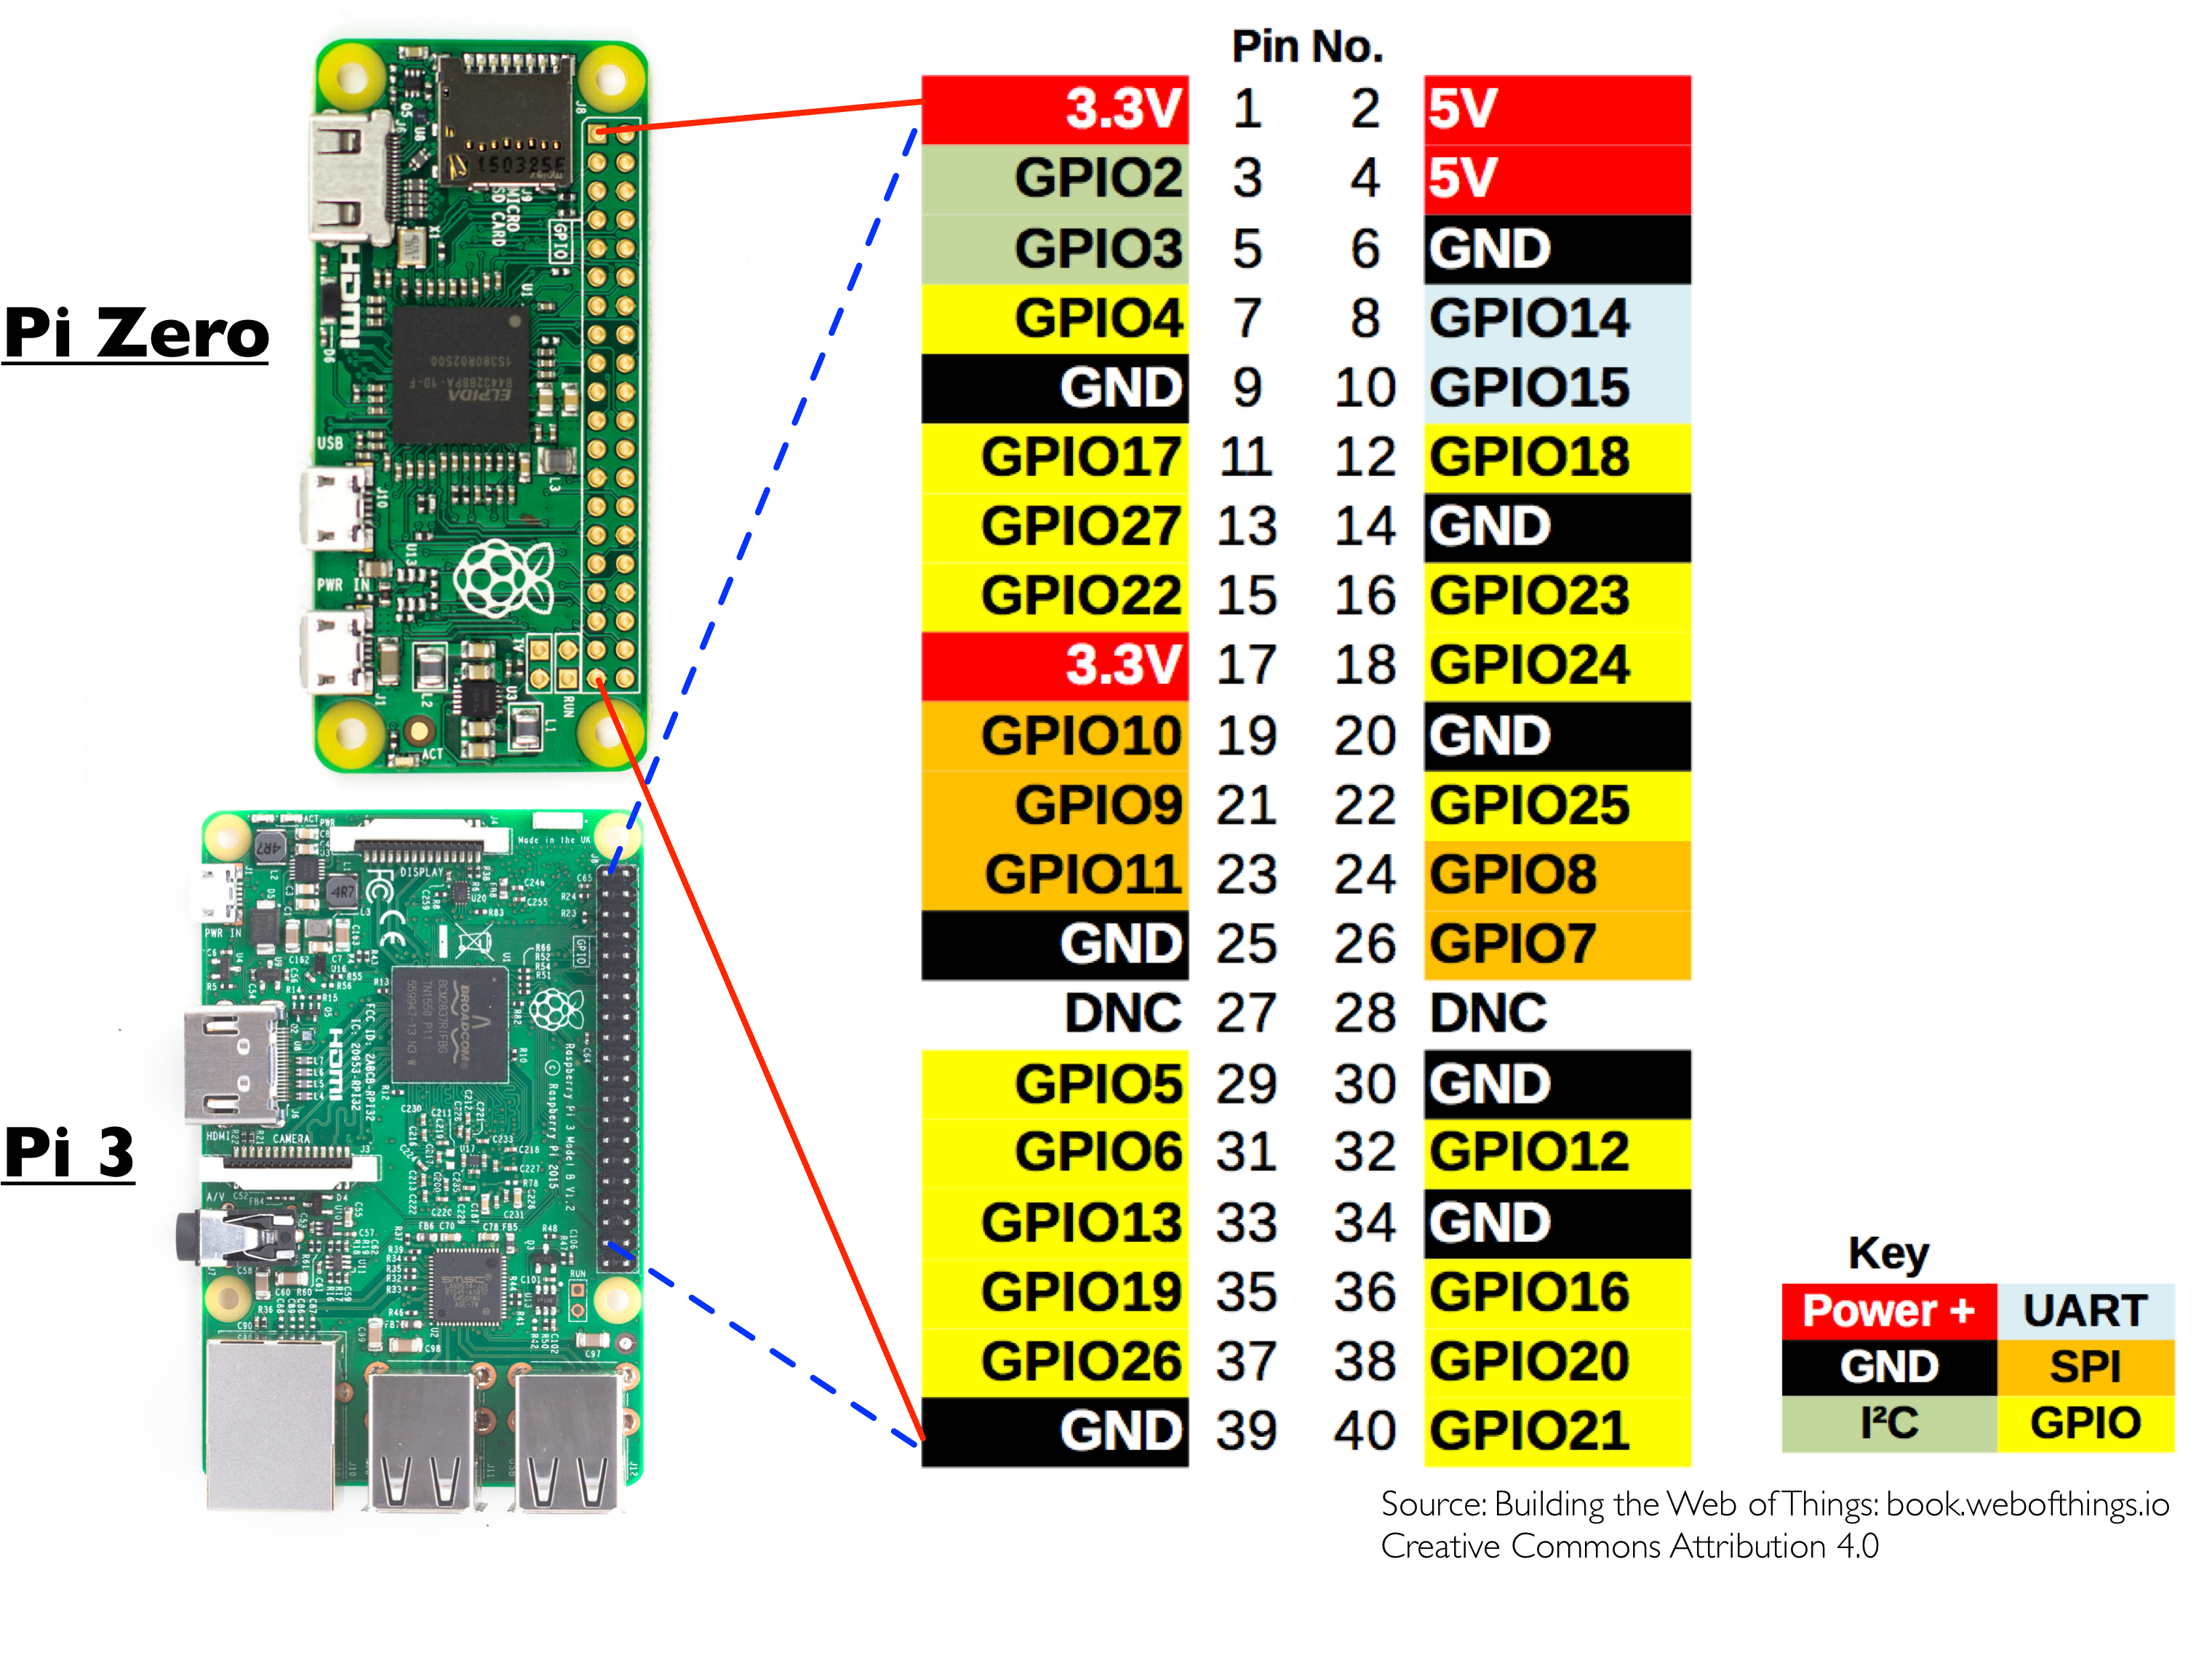
\includegraphics[width=1\textwidth,page=1]{pi}
    \caption{RaspberryPi and GPIO circuit}
    \label{RaspberryPi}
\end{figure}

\begin{figure}[htp]
    \centering
    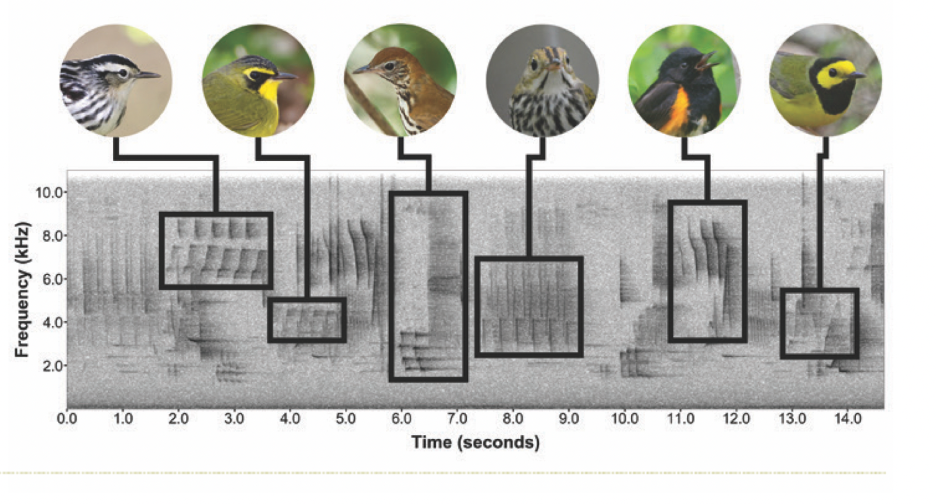
\includegraphics[width=1\textwidth,page=1]{birdCalls}
    \caption{Recognizing bird call frequencies with AudioMoth}
    \label{BirdCalls}
\end{figure}

\pagebreak




\end{document}